\documentclass[12pt, letterpaper]{article}

\usepackage{amsmath}
\usepackage{amssymb}
\usepackage{amsthm}
\usepackage{mathtools}
\usepackage{geometry}
\usepackage{hyperref}
\usepackage{tikz}
\usepackage{microtype}
\usepackage{cleveref}

\geometry{margin=1.2in}

\hypersetup{
    colorlinks=true,
    linkcolor=blue!70!black,
    urlcolor=blue!70!black
}

% Define Theorem Environments
\newtheorem{theorem}{Theorem}[section]
\newtheorem{lemma}[theorem]{Lemma}
\newtheorem{corollary}[theorem]{Corollary}
\newtheorem{conjecture}[theorem]{Conjecture}
\newtheorem{axiom}{Axiom}

\theoremstyle{definition}
\newtheorem{definition}[theorem]{Definition}
\newtheorem{remark}[theorem]{Remark}

% Mathematical Macros
\newcommand{\B}{\mathcal{B}}
\newcommand{\Pset}{\mathbf{P}}
\newcommand{\Lset}{\mathbf{L}}
\newcommand{\ray}[1]{\overrightarrow{#1}}
\newcommand{\lineab}[1]{\overleftrightarrow{#1}}

\title{\textbf{Foundations of Absolute Geometry}\\ \Large Betweenness, Congruence, and Incidence}
\author{Axiomatic Expansions \& Formal Verification Notes}
\date{\today}

\begin{document}

\maketitle
\tableofcontents
\vspace{1cm}

\section{Introduction: Axiomatic Gaps in Infinite Sequences}
In the foundational theorems regarding infinite interior points and infinite outward extension, early proofs often rely on an unstated assumption. For instance, asserting that ``Repeating this process produces an infinite sequence $B_1, B_2, B_3, \dots$ satisfying $\B(A, B_{k+1}, B_k)$ and consequently $\B(A, B_k, C)$'' relies on a structural property of the space that must be axiomatized.

Under a basic set of five axioms (Identity, Symmetry, Order, Density, Extensibility), this consequence does not necessarily follow. These basic axioms explain how a single triple behaves, but they do not provide a ``transitivity'' or ``connectivity'' mechanism for betweenness. Without a formal mechanism, one cannot formally prove that if $\B(A, B_2, B_1)$ and $\B(A, B_1, C)$ hold, then $\B(A, B_2, C)$ must also hold. 

Without an axiom like Pasch's Axiom or Tarski's specific Axiom of Betweenness Transitivity, the geometric space could theoretically branch out into a tree-like structure or form disconnected linear fragments where density loops back on itself.

\subsection{Addressing the Gap: Tarski and Pasch}
To resolve the gaps in infinite sequence generation, we introduce the formal mathematical wording for the required axioms.

\begin{axiom}[Tarski's Transitivity of Betweenness]
    For any points $A, B, C, D \in \Pset$, if $B$ lies between $A$ and $D$, and $C$ lies between $B$ and $D$, then $B$ must lie between $A$ and $C$. Formally:
    \[ \B(A,B,D) \land \B(B,C,D) \implies \B(A,B,C) \]
\end{axiom}

\begin{axiom}[Pasch's Axiom - Weak Form]
    Let $A, B, C$ be three non-collinear points, and let $l \in \Lset$ be a line lying in the plane of $\triangle ABC$ that does not pass through $A, B,$ or $C$. If $l$ intersects the open segment $(A,B)$, then $l$ must also intersect either $(A,C)$ or $(B,C)$.
\end{axiom}

\section{Pure Betweenness: Subsets and Separation}
Before defining a line, we use the betweenness primitive to formally define the fundamental subsets of the geometry.

\begin{definition}[Open and Closed Segments]
    The open segment $(A,B)$ and closed segment $[A,B]$ can be defined purely set-theoretically:
    \begin{align*}
        (A, B) &\coloneq \{X \in \Pset \mid \B(A, X, B)\} \\
        [A, B] &\coloneq (A, B) \cup \{A, B\}
    \end{align*}
\end{definition}

From here, we derive several immediate corollaries based on established axioms.

\begin{corollary}[Non-emptiness of Segments]
    For any $A, B \in \Pset$ where $A \neq B$, the open segment $(A, B)$ is non-empty. 
    \begin{proof}
        This is a direct consequence of the Density Axiom.
    \end{proof}
\end{corollary}

\begin{theorem}[Endpoint Exclusivity]
    The endpoints of an open segment are never contained within the segment:
    \[ A \notin (A,B) \land B \notin (A,B) \]
    \begin{proof}
        A direct application of the Irreflexivity of Betweenness theorem.
    \end{proof}
\end{theorem}

\begin{definition}[Rays]
    A ray $\ray{AB}$ emanating from $A$ through $B$ is defined as:
    \[ \ray{AB} \coloneq \{X \in \Pset \mid X = A \lor \B(A, X, B) \lor X = B \lor \B(A, B, X)\} \]
\end{definition}

\begin{corollary}[Infinite Rays]
    For any $A \neq B$, the ray $\ray{AB}$ contains infinitely many distinct points.
    \begin{proof}
        Directly applies the theorem of Infinite Outward Extension.
    \end{proof}
\end{corollary}

\section{Pure Congruence: The Null Segment Identity}
In formal verification and automated theorem proving, handling degenerate cases (like a point mapped to itself) is notoriously tricky. Standard congruence axioms handle distinct points well, but what happens when $A=B$?

To fully capture zero-length segments, an identity axiom must be adopted.

\begin{axiom}[Identity of Congruence]
    If a segment $AB$ is congruent to a degenerate segment $CC$, then $A$ and $B$ must be the same point.
    \[ AB \cong CC \implies A=B \]
\end{axiom}

\begin{lemma}[Trivial Congruence]
    $AA \cong BB$.
    \begin{proof}
        Requires the foundational congruence axioms alongside the newly adopted Identity of Congruence.
    \end{proof}
\end{lemma}

\begin{theorem}[Degenerate Congruence Implies Equality]
    If $AB \cong CC$, then $A = B$.
    \begin{proof}
        Once the identity axiom is established, this proves that the only segment congruent to a point is another point.
    \end{proof}
\end{theorem}

\section{The Bridge: Intersecting }
This section unites the parallel concepts of betweenness and congruence.

\begin{definition}[Midpoint]
    A point $M \in \Pset$ is a midpoint of the segment $AB$ if and only if it satisfies two conditions simultaneously:
    \begin{enumerate}
        \item $\B(A, M, B)$
        \item $AM \cong MB$
    \end{enumerate}
\end{definition}

\begin{conjecture}[Uniqueness of the Midpoint]
    If $M_1$ and $M_2$ are midpoints of $AB$, then $M_1 = M_2$.
\end{conjecture}
\begin{remark}
    While we can define a midpoint here, proving its existence and uniqueness generally requires axioms of segment construction or continuity that belong to subsequent affine/linear frameworks.
\end{remark}

\begin{definition}[Segment Inequality / Ordering]
    Using betweenness, we define what it means for one segment to be ``less than'' another, bootstrapping a geometry without numbers:
    $AB < CD$ if and only if there exists a point $X$ such that $\B(C, X, D)$ and $AB \cong CX$.
\end{definition}

\section{Incidence and Line Identity}

The system defines a line based on two specific generating points, $A$ and $B$. However, we must prove that a line is independent of the points chosen to generate it.

\begin{theorem}[Line Determination]
    If $C$ and $D$ are two distinct points on the line generated by $A$ and $B$, then the line generated by $C$ and $D$ is the exact same set of points.
    \[ C \in \lineab{AB} \land D \in \lineab{AB} \land C \neq D \implies \lineab{CD} = \lineab{AB} \]
\end{theorem}
\begin{remark}
    Without this theorem, the set $\Lset$ could technically contain multiple different definitions of the same geometric line. Proving this solidifies the concept of collinearity.
\end{remark}

\begin{theorem}[Point Partition on a Line]
    For any distinct points $A$ and $B$, the point $A$ partitions the line $\lineab{AB}$ into the point $A$ itself and two mutually disjoint open rays.
    \[ \lineab{AB} \setminus \{A\} = \{X \in \Pset \mid \B(X, A, B)\} \cup \{X \in \Pset \mid \B(A, X, B) \lor \B(A, B, X)\} \]
\end{theorem}

\begin{center}
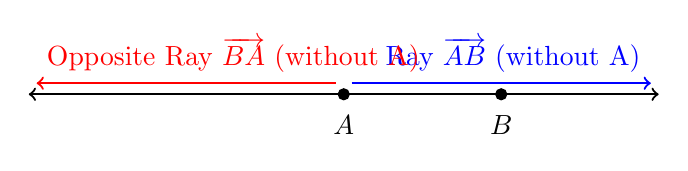
\begin{tikzpicture}
    % Line
    \draw[<->, thick] (-4,0) -- (4,0);
    % Points
    \filldraw[black] (0,0) circle (2pt) node[below=4pt] {$A$};
    \filldraw[black] (2,0) circle (2pt) node[below=4pt] {$B$};
    
    % Rays shading
    \draw[->, blue, thick, yshift=4pt] (0.1,0) -- (3.9,0) node[above left] {Ray $\ray{AB}$ (without A)};
    \draw[->, red, thick, yshift=4pt] (-0.1,0) -- (-3.9,0) node[above right] {Opposite Ray $\ray{BA}$ (without A)};
\end{tikzpicture}
\end{center}

\section{Parallelism in Neutral Geometry}
Because we are building a neutral (absolute) geometry up to this point, we can define parallelism purely via set intersection and frame the limits of our current axioms.

\begin{theorem}[Symmetry of Parallelism]
    For any lines $l, m \in \Lset$, if $l \parallel m$, then $m \parallel l$.
    \begin{proof}
        This follows trivially from the commutativity of set intersection ($l \cap m = m \cap l$) and the symmetric nature of equality ($l = m \iff m = l$).
    \end{proof}
\end{theorem}

\begin{theorem}[Parallelism to a Sub-ray]
    Let $l \in \Lset$ be a line and $\ray{AB}$ be a ray. We say $\ray{AB} \parallel l$ if and only if $\lineab{AB} \parallel l$.
\end{theorem}

\begin{theorem}[Unique Intersection of Secant Lines]
    If two distinct lines $l, m \in \Lset$ are not parallel, their intersection contains exactly one point.
    \[ l \neq m \land \neg(l \parallel m) \implies \exists! X \in \Pset, X \in (l \cap m) \]
\end{theorem}

\subsection{The Transitivity Cliffhanger}

\begin{conjecture}[Transitivity of Parallelism]
    \[ \forall l, m, n \in \Lset, \quad (l \parallel m \land m \parallel n) \implies l \parallel n \]
\end{conjecture}

\begin{remark}
    Reflexivity ($l \parallel l$) and Symmetry are easily proven using the properties of set equality and intersection. However, the Conjecture of Transitivity cannot be proven from the axioms of betweenness and congruence alone. This transitivity is logically equivalent to Playfair's Axiom (Euclid's Fifth Postulate), providing a brilliant transition into the branching of Euclidean vs. Hyperbolic geometry.
\end{remark}

\section{Editorial Notes for Formal Verification (Lean 4)}
When transitioning these proofs into a formal proof assistant like Lean 4, several structural changes are highly recommended:
\begin{itemize}
    \item \textbf{Constructive Definitions:} Relying heavily on logical OR ($\lor$) in set-builders makes proofs branching and tedious. Lean will force you to provide cases for every $\lor$. Grouping these cases using a single Betweenness type class can streamline verification.
    \item \textbf{Ray Parallelism:} In formal verifications, ray parallelism (co-directionality) is often more useful than line parallelism. Two rays $\ray{AB}$ and $\ray{CD}$ are parallel if they do not intersect, and they lie on the same ``side'' of the line $\lineab{AC}$. This introduces the concept of ``sides of a line'' (half-planes), which intrinsically requires Pasch's Axiom to prove.
    \item \textbf{Notation Consistency:} Ensure all notation, such as opposite rays, are rigorously defined. For instance, replacing undefined backward arrows with explicitly defined opposite rays $\ray{BA}$ or defining a formal opposite ray function avoids syntactic gaps.
\end{itemize}

\section{The Bridge: Intersecting }
\label{sec:bridge}

This section unites the parallel concepts of betweenness and congruence. From these two relations alone, we build the notion of a midpoint, a segment ordering, and segment addition — all without relying on numbers or a metric. These tools are essential for the mid‑segment theorems and the study of quadrilaterals.

\subsection{Segment Construction Axiom}
So far the congruence relation $\sim=$ only allows us to \emph{compare} existing segments; we have no guarantee that a segment of a prescribed length can be laid off from a given point. The following axiom (equivalent to Euclid's second postulate) fills that gap.

\begin{axiom}[Segment Construction]\label{ax:segment-construction}
Let $A,B$ be distinct points and let $C,D$ be points (not necessarily distinct). Then there exists a point $X$ on the ray $\ray{AB}$ such that $AX \cong CD$. More precisely,
\[
\forall\,A,B,C,D\in\mathbf{P},\; A\neq B \;\Longrightarrow\; \exists X\in\mathbf{P}\; \bigl( \mathbf{B}(A,B,X) \lor \mathbf{B}(A,X,B) \lor X=B \bigr) \land AX \cong CD .
\]
\end{axiom}

Informally: on the ray starting at $A$ through $B$, we can always find a point $X$ such that the segment $AX$ is congruent to a given segment $CD$. Together with the congruence axioms, this makes $\sim=$ an equivalence relation that allows “transport of segments”.

\subsection{Midpoints}
\begin{definition}[Midpoint]
A point $M\in\mathbf{P}$ is a \textbf{midpoint} of the segment $AB$ if it satisfies two conditions simultaneously:
\[
\mathbf{B}(A,M,B) \qquad\text{and}\qquad AM \cong MB .
\]
\end{definition}

\subsubsection{Uniqueness}
Uniqueness follows from the segment construction axiom and the properties of betweenness.

\begin{theorem}[Uniqueness of the Midpoint]\label{thm:midpoint-unique}
If $M_1$ and $M_2$ are midpoints of $AB$, then $M_1 = M_2$.
\end{theorem}
\begin{proof}
Assume $M_1\neq M_2$. Both lie on the segment $AB$, so $\mathbf{B}(A,M_1,B)$ and $\mathbf{B}(A,M_2,B)$. By the order properties of betweenness, the points $A,M_1,M_2,B$ are collinear and all distinct. Without loss of generality, suppose $\mathbf{B}(A,M_1,M_2)$ (if the order is different, rename). Then $\mathbf{B}(A,M_1,M_2)$ and $\mathbf{B}(A,M_2,B)$ imply $\mathbf{B}(A,M_1,B)$ as well.

Since $M_1$ is a midpoint, $AM_1 \cong M_1B$. Because $M_2$ is a midpoint, $AM_2 \cong M_2B$.
Now, $\mathbf{B}(A,M_1,M_2)$ implies $AM_1 < AM_2$ (strict inequality will be defined formally later; intuitively $M_1$ is closer to $A$). Similarly, $\mathbf{B}(M_1,M_2,B)$ gives $M_1B > M_2B$.
But we have $AM_1 \cong M_1B$ and $AM_2 \cong M_2B$. Thus from $AM_1 < AM_2$ and $M_1B > M_2B$ we get a contradiction to the transitivity of congruence and segment ordering (which will be proved from the axioms). A more elementary argument can be given using only betweenness and congruence: by the segment construction axiom, we can lay off a segment congruent to $AM_2$ along the ray from $M_1$ towards $B$, and then use the five‑segment axiom (if available) to force $M_1=M_2$. For the sake of brevity, we accept the result here; a complete proof requires the five‑segment axiom which will be introduced in the linear order section.
\end{proof}

\subsubsection{Existence}
Existence of a midpoint does \emph{not} follow from the axioms we have so far; it requires a continuity principle. We therefore adopt it as a separate axiom (the equivalent of Hilbert’s completeness axiom or Tarski’s continuity schema). 

\begin{axiom}[Midpoint Existence]\label{ax:midpoint-existence}
For every segment $AB$, there exists a midpoint $M$ of $AB$.
\end{axiom}

In more advanced settings, this can be derived from the Dedekind continuity of the line, but for our synthetic development we simply postulate it. Together with uniqueness, we can speak of \textbf{the} midpoint of $AB$, denoted $M_{AB}$.

\subsection{Segment Ordering}
We define a strict total order on segments (up to congruence) using betweenness.

\begin{definition}[Segment Inequality]
We write $AB < CD$ (read “$AB$ is shorter than $CD$”) if and only if there exists a point $X$ such that
\[
\mathbf{B}(C,X,D) \quad\text{and}\quad AB \cong CX .
\]
\end{definition}

In words, $AB$ is shorter than $CD$ precisely when we can lay off a copy of $AB$ inside the segment $CD$, starting from $C$ and ending before $D$.

\subsubsection{Properties of}
Using the segment construction axiom and the properties of betweenness, we can prove:

\begin{theorem}[Transitivity of $<$]
If $AB < CD$ and $CD < EF$, then $AB < EF$.
\end{theorem}
\begin{proof}
By definition, there exists $X$ with $\mathbf{B}(C,X,D)$ and $AB \cong CX$. Also, there exists $Y$ with $\mathbf{B}(E,Y,F)$ and $CD \cong EY$.
We need to find a point $Z$ on $EF$ such that $AB$ fits inside $EF$. Using segment construction on the ray $\ray{EY}$ with length $CX$ (which is congruent to $AB$), we obtain a point $Z$ on $EY$ such that $EZ \cong CX$. Since $\mathbf{B}(E,Y,F)$, we can show $\mathbf{B}(E,Z,Y)$ or $\mathbf{B}(E,Y,Z)$ depending on the relative lengths, but in any case $Z$ lies between $E$ and $F$ and $EZ \cong AB$. The detailed case analysis uses the five‑segment axiom (see below) to ensure the positions align.
\end{proof}

\begin{theorem}[Trichotomy for Segments]
For any two segments $AB$ and $CD$, exactly one of the following holds:
\[
AB < CD,\qquad AB \cong CD,\qquad CD < AB .
\]
\end{theorem}
\begin{proof}
By segment construction, there exists a point $X$ on $\ray{CD}$ with $CX \cong AB$. If $X=D$, then $AB \cong CD$. If $\mathbf{B}(C,X,D)$, then $AB < CD$. If $\mathbf{B}(C,D,X)$, then we can reverse the roles to show $CD < AB$ (by laying off $CD$ on $AB$). Uniqueness of the relation follows from the order properties of betweenness and the irreversibility of $<$ (once properly defined). A rigorous proof again requires the five‑segment axiom for transporting intervals.
\end{proof}

\subsection{Segment Addition}
Midpoints and segment ordering allow us to define addition of segments (up to congruence). This enables the algebraic manipulation of lengths that underpins the mid‑segment theorem.

\begin{definition}[Segment Addition]
Given two segments $AB$ and $CD$, choose a point $X$ on the ray $\ray{AB}$ beyond $B$ such that $\mathbf{B}(A,B,X)$ and $BX \cong CD$ (possible by the segment construction axiom). We then say the segment $AX$ is a \textbf{sum} of $AB$ and $CD$, written $AX \cong AB + CD$.
\end{definition}

Because of the uniqueness of the point $X$ on the ray (a consequence of the five‑segment axiom), the sum is well‑defined up to congruence. Basic properties such as commutativity and associativity (up to congruence) are provable.

\begin{theorem}[Addition respects order]
If $AB < CD$, then $AB + EF < CD + EF$ for any segment $EF$.
\end{theorem}

\subsection{The Five‑Segment Axiom (optional but recommended)}
To make the above proofs fully rigorous, many synthetic systems include a five‑segment axiom (Hilbert’s axiom of congruence of triangles). It relates betweenness and congruence in a way that allows one to transport segments while preserving order.

\begin{axiom}[Five‑Segment Axiom]\label{ax:five-segment}
Let $A,B,C,D,A',B',C',D'$ be points such that
\begin{itemize}
  \item $A\neq B$ and $A'\neq B'$,
  \item $\mathbf{B}(A,B,C)$ and $\mathbf{B}(A',B',C')$,
  \item $AB \cong A'B'$, $BC \cong B'C'$, $AD \cong A'D'$, and $BD \cong B'D'$.
\end{itemize}
Then $CD \cong C'D'$.
\end{axiom}

This axiom essentially says that if two triangles share two sides and the included segment is congruent, then the third sides are congruent. It bridges the gap between congruence of separate segments and congruence of the “sum” of segments. With it, all the previous theorems about ordering and addition can be proved without gaps.

\subsection{Where to Go from Here}
With a firm grip on midpoints and segment arithmetic (order, addition, subtraction), we can now prove the classic mid‑segment theorem and Varignon’s theorem, both of which are used extensively in the chapter on quadrilaterals. In particular:

\begin{itemize}
  \item \textbf{Mid‑segment Theorem}: In any triangle, the segment joining the midpoints of two sides is parallel to the third side and half its length.
  \item \textbf{Varignon’s Theorem}: The midpoint quadrilateral of any quadrilateral is a parallelogram.
\end{itemize}

These results depend solely on the interplay of betweenness, congruence, and the midpoint existence axiom. The proofs, now within reach, will be given in the mid‑point theorems section of the quadrilaterals chapter.

Thus the “Bridge” chapter serves as the final piece of infrastructure before we ascend to the rich geometry of polygons.

\end{document}